\section{High level description of components}
%TODO (Lucas): Rework high level
%TODO (Lucas): Improve graphic

The components of Centrifuge are a collection of Ethereum Smart Contracts and a peer to peer network implemented on libp2p\footnote{\url{https://github.com/libp2p/specs}} (see Fig. \ref{fig:high_level_architecture}). Ethereum smart contracts are used for maintaining identities in a similar format to the ERC725 standard\footnote{\url{https://github.com/ethereum/EIPs/blob/master/EIPS/eip-725.md}}. There is a contract deployed to store state commitments and a standard way of minting NFTs\footnote{\url{https://github.com/ethereum/EIPs/blob/master/EIPS/eip-721.md}} from off chain Centrifuge documents.
\begin{figure}[thpb]
  \centering
  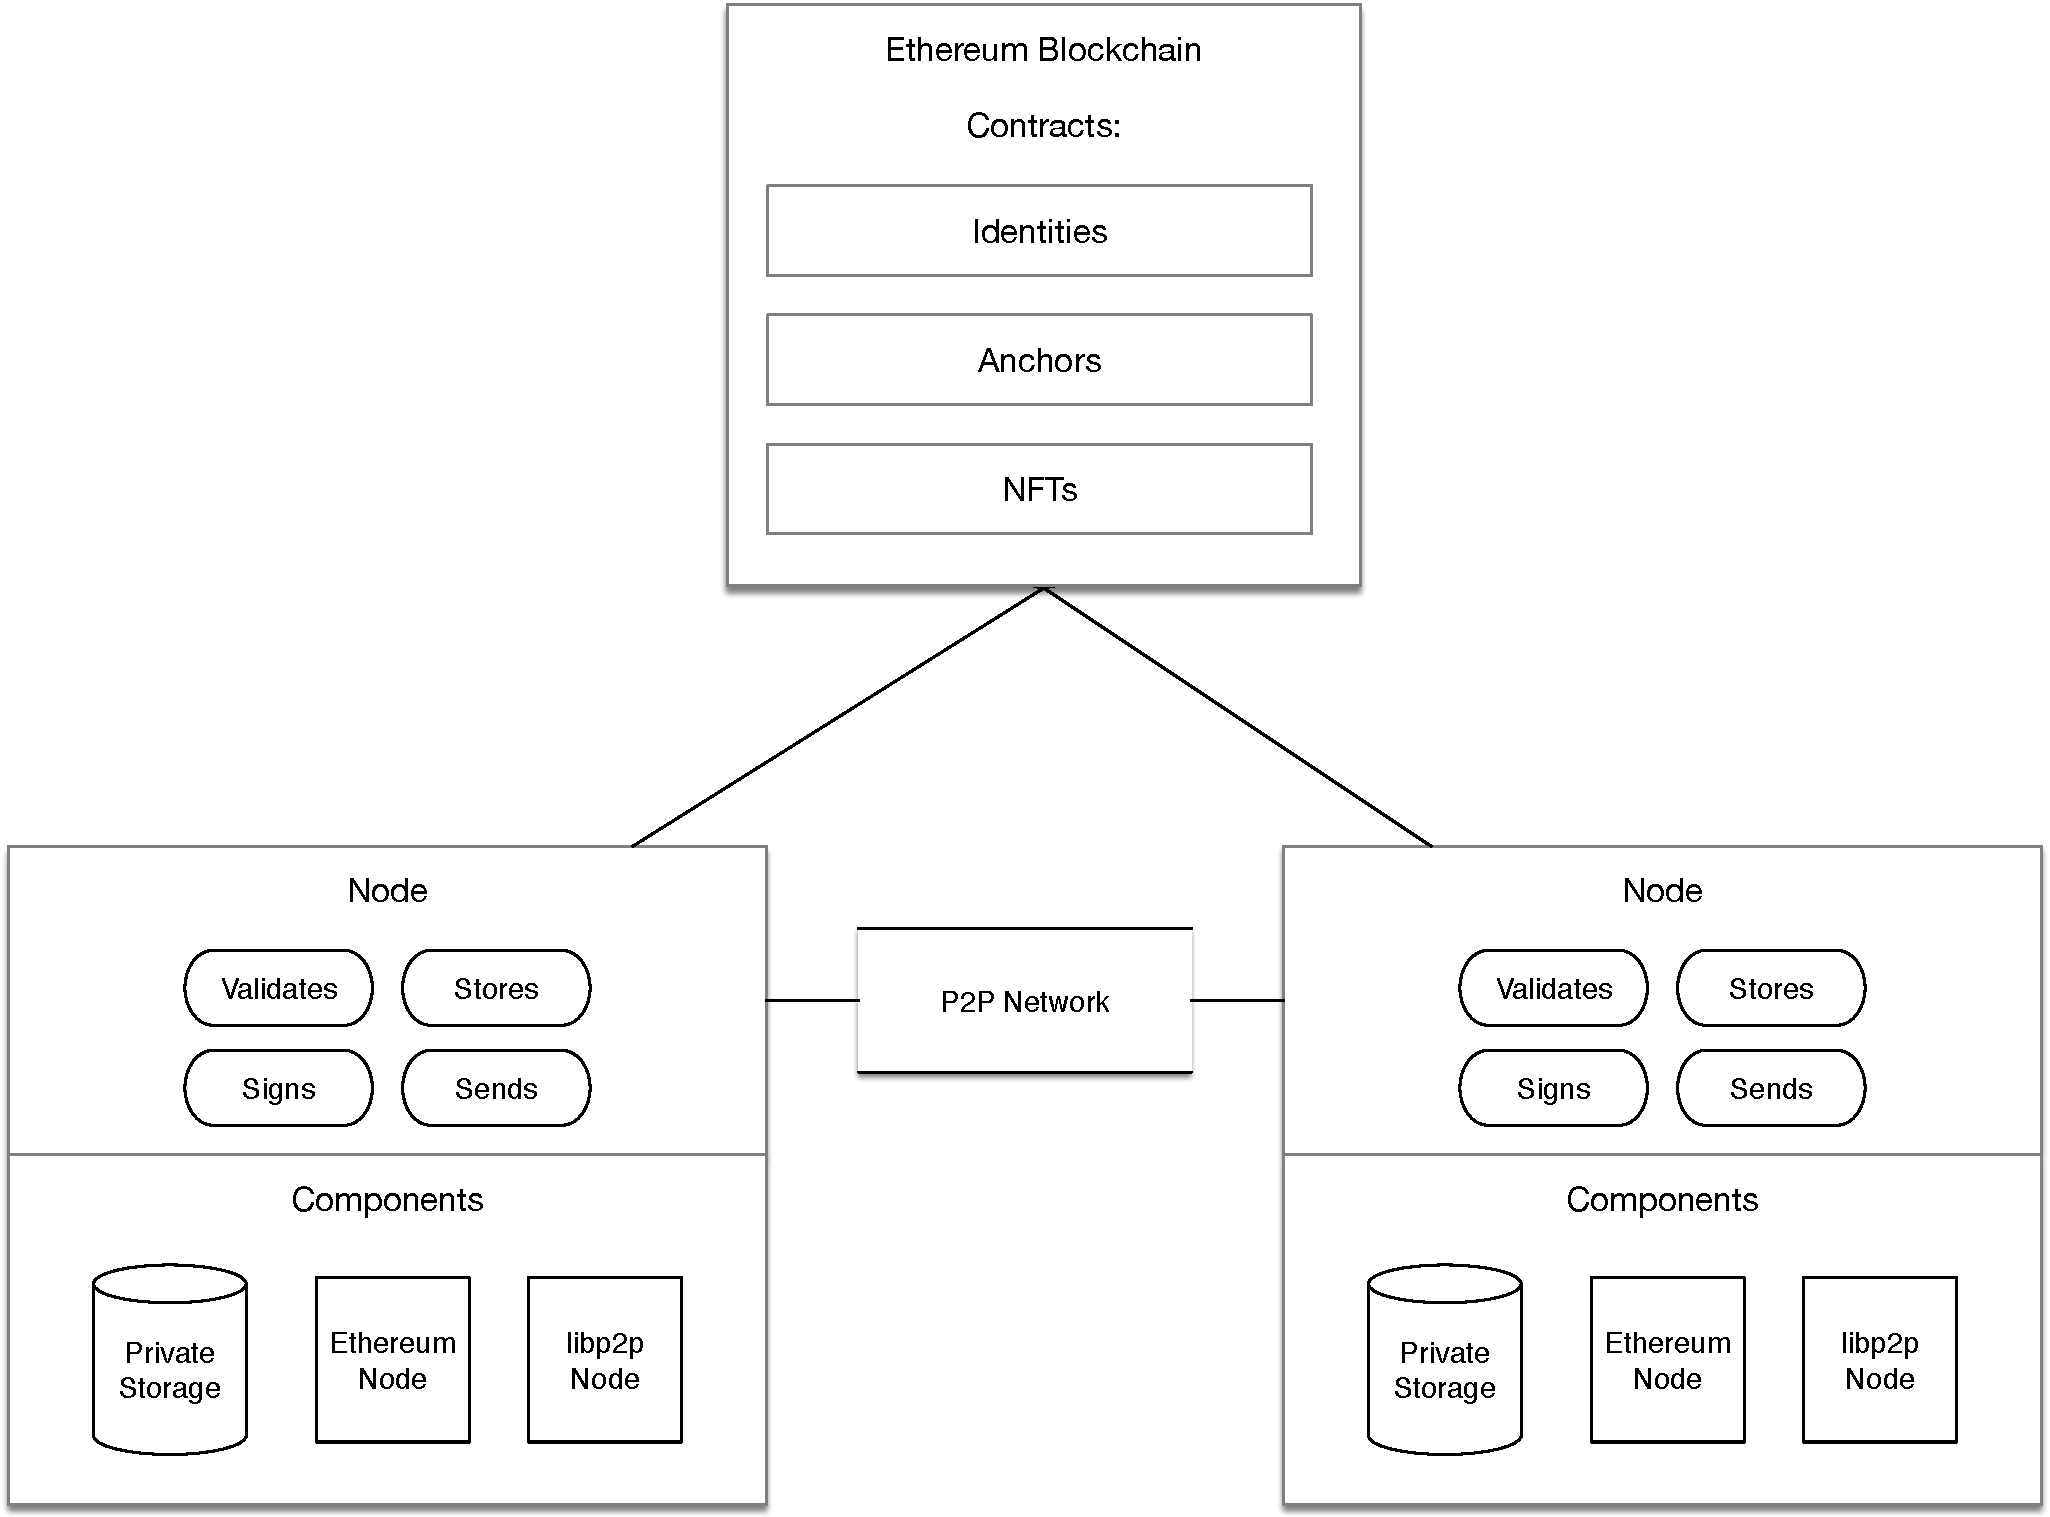
\includegraphics[width=11cm]{img/high_level_architecture.pdf}
  \caption{Overview of the components making up the Centrifuge protocol} 
  \label{fig:high_level_architecture}
\end{figure}

\subsection{Ethereum \& P2P}
% TODO: Extend this section a bit
Centrifuge is a P2P protocol built on libp2p to exchange information privately without a trusted third party or intermediary. Ethereum is used as a blockchain where necessary.

\subsection{Identity}
A node in the Centrifuge protocol uses different key pairs for signing documents and for authentication on the p2p layer. A user-deployed identity contract keeps the latest public keys. New keys can only be added by the user, and the contract can verify signatures on-chain. The identity contract thus represents the self sovereign identity of a user, as well as acting as a proxy contract for interaction with other on-chain decentralized applications. Centrifuge is adopting the DID-compatible ERC725 standard for identities.

\subsection{Documents}
A document is a well-known, structured set of fields with specific types. The protocol supports any document types as long as the formats are agreed upon and shared between the participants of a participant set-- e.g. a document can be an invoice with agreed upon fields and line items, or a purchase order. The structure of the document becomes important for reaching consensus by attaching signatures to the document state, as well as creating specific attestations about a document at a later point in time. Documents are exchanged encrypted, and are only accessible for parties involved in this private data exchange. Collaborators can be added and removed from a document. Different collaborators can update a document and publish new versions within the set of nodes with access.
A smart contract called \textit{AnchorRepository} is used for carbon dating state updates and serves as a bulletin board\cite{heiberg2018trade} to ensure that the update is made known to all collaborators. A document anchor is the root hash of the Merkle tree of the document. The tree is constructed by adding all fields of a document together with the collected signatures from all collaborators as leaves in the tree. Publishing this anchor achieves that even if a party is censored on the P2P network, it can find out about the update by checking the Ethereum blockchain.
A third party can easily verify the correctness of a received document on-chain and off-chain by reconstructing the Merkle root from the document based on the well-known document structure for the respective document type. Structuring the document as a Merkle tree allows creation of proofs only revealing individual fields of the document as opposed to revealing the entire document when making a statement about it.

\subsection{NFT - Non Fungible Tokens}
An integral part of Centrifuge is interaction with other applications built on Ethereum. One way to interact with the greater ecosystem is through NFTs. Centrifuge uses privacy-enabled NFTs\cite{centrifuge2018nft} to allow for minting of NFTs that have verified attributes from private documents. The Merkle proofs that refer to a state commitment published in our \textit{AnchorRepository} contract immutably link the NFT to an off-chain document.

